\section{Rechnung an einem konkreten Beispiels}

\subsection{Brechungsgesetz von Snellius \label{brechungsgesetz}}
\cite{Wikipedia} Aus dem Fermatschen Prinzip lässt sich das Brechungsgesetz von Snellius herleiten.
Das Licht legt den Weg vom Startpunkt $P_0$ über den Brechungspunkt $P_1$ 
nach dem Endpunkt $P_2$ zurück, siehe \figref{Ab:brechung}.
\begin{figure}[H]
\begin{center}
	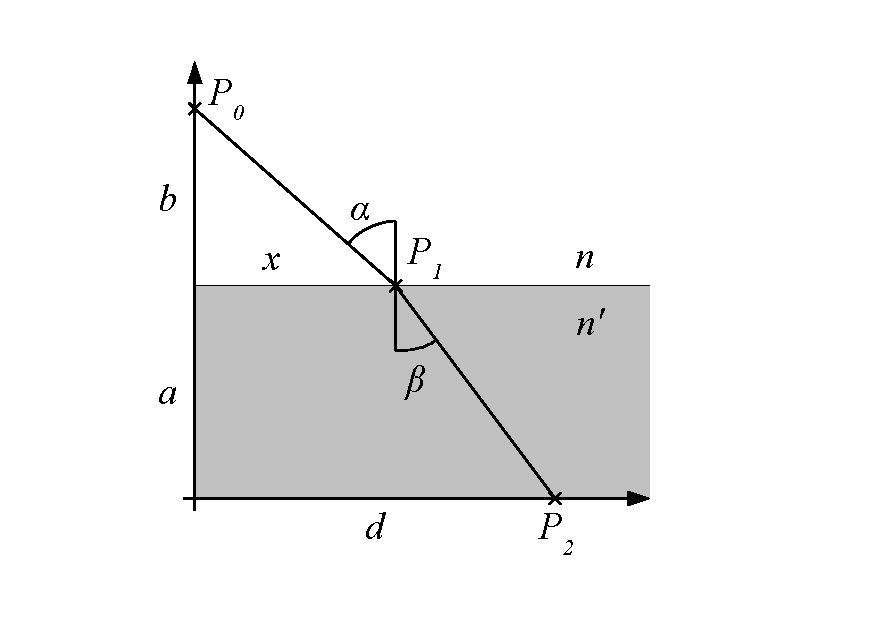
\includegraphics[width=0.7\textwidth]{./picture/Brechung.pdf}
	\caption{Skizze des Brechungsgesetzes von Snellius}
	\label{Ab:brechung}
\end{center}
\end{figure}

Dadurch kann die zurückgelegte Zeit berechnet werden (\eqref{snelliusT}).
\begin{align}
t(x) = t_1 + t_2 = \frac{s_1}{c_1} + \frac{s_2}{c_2} = \frac{|P_1 - P_0|}{c_1} + \frac{|P_2 - P_1|}{c_2} \notag \\
= \frac{\sqrt{a^2 + x^2}}{c_1} + \frac{\sqrt{(d-x)^2 + b^2}}{c_2} \label{snelliusT}
\end{align}

Wird diese Funktion nach $dx$ abgeleitet und gleich Null gesetzt wird, die Extremastelle von $t$ gefunden (\eqref{snelliusDx}).
\begin{align}
	\frac{dt}{dx} = \frac{2 \cdot x}{2 \cdot c_1 \cdot \sqrt{a^2 + x^2}} + \frac{-2 \cdot (d-x)}{2 \cdot c_2 \cdot \sqrt{(d-x)^2 + b^2}} \notag \\
	= \frac{x}{c_1 \cdot \sqrt{a^2 + x^2}} - \frac{(d-x)}{c_2 \cdot \sqrt{(d-x)^2 + b^2}} = 0 
	\label{snelliusDx}
\end{align}

Hier wird auf den Beweis das es ein Minima ist verzichtet, da es riesige Terme gibt um $x_0$ in Abhängigkeit von den anderen Konstanten und deren Nebenbedingungen auszudrücken.

Aus \figref{Ab:brechung} ist gut ersichtlich, dass die Substitutionen \ref{substitution1} und \ref{substitution2} durchgeführt werden können.

\begin{align}
	\sin(\alpha) &= \frac{x}{\cdot \sqrt{a^2 + x^2}}  \label{substitution1}\\
	\sin(\beta) &= \frac{d-x}{\sqrt{(d -x)^2 + b^2}} \label{substitution2}
\end{align}

Nach etwas umformen ergibt sich das Verhältnis der Winkel $\alpha \ \text{und} \ \beta$ gemäss (\eqref{snellius}).

\begin{equation}
	0 = \frac{\sin(\alpha)}{c_1} - \frac{\sin(\beta)}{c_2} \Leftrightarrow\frac{c_2}{c_1} = \frac{\sin(\beta)}{\sin(\alpha)}
	\label{snellius}
\end{equation}


\subsection{Reflexionsgesetz}
\cite{Wikipedia} Auf gleiche weise, wie das das Brechungsesetz aus dem Fermatschen Prinzip hergeleitet wird, 
lässt sich daraus auch das Reflexionsgesetz ableiten.
Das Licht legt den Weg vom Startpunkt $P_0$ über den Spiegelpunkt $P_1$ 
nach dem Endpunkt $P_2$ zurück. Dadurch kann die zurückgelegte Zeit berechnet werden (\eqref{reflexion}).


\begin{align}
t(x) = t_1 + t_2 &= \frac{s_1 + s_2}{c} = \frac{|P_1 - P_0| + |P_2 - P_1|}{c} \notag \\
&= \frac{\sqrt{a^2 + x^2} + \sqrt{(d-x)^2 + b^2}}{c} \label{reflexion}
\end{align}

Wenn $t(x)$ nach $dx$ abgeleitet und gleich 0 gesetzt wird, ergibt sich die Extremastelle  von $t$ (\eqref{reflexionDx}). Auf den Beweis, dass es ebenfalls ein Minimum ist, wie bei der Reflexion, wird hier verzichtet.

\begin{align}
\frac{dt}{dx} &= \frac{1}{c} \cdot \frac{2 \cdot x}{2 \cdot \sqrt{a^2 + x^2}} + \frac{-2 \cdot (d-x)}{2 \cdot \sqrt{(d-x)^2 + b^2}} \notag \\
&= \frac{x}{ \sqrt{a^2 + x^2}} - \frac{(d-x)}{ \sqrt{(d-x)^2 + b^2}} = 0 \label{reflexionDx}
\end{align}


In \figref{Ab:spiegelung} ist ersichtlich, dass die Substitutionen \ref{substitution1} und \ref{substitution2} von \secref{brechungsgesetz} auch hier nützlich sind.
Nach etwas umformen ergibt sich, dass Eintritts- und Austrittswinkel gleich sind (\eqref{brechung}).


\begin{equation}
0 = \sin(\alpha) - \sin(\beta) \quad \Leftrightarrow \quad \sin(\beta) = \sin(\alpha) \quad \Leftrightarrow\quad \beta = \alpha
\label{brechung}
\end{equation}

\begin{figure}[H]
\begin{center}
	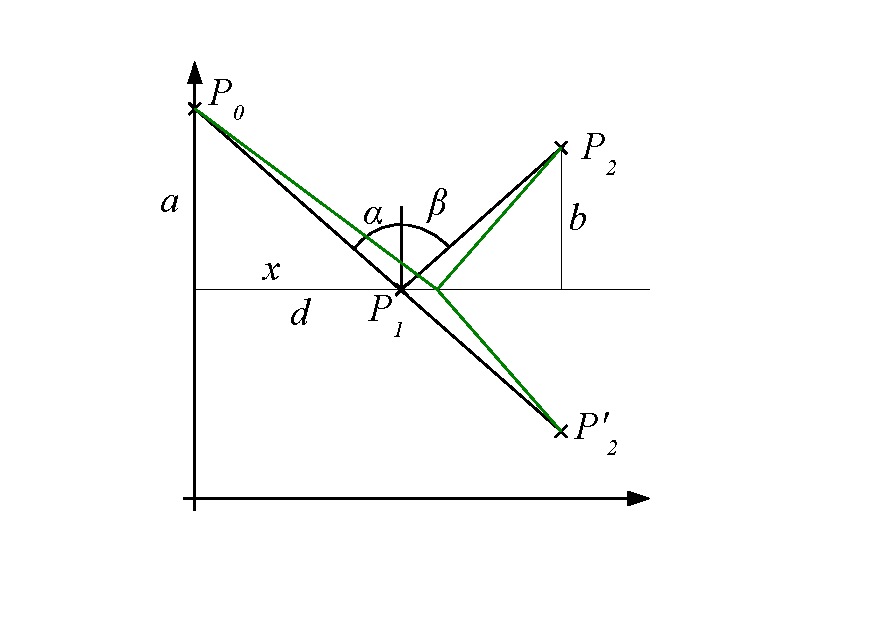
\includegraphics[width=0.7\textwidth]{./picture/Spiegelung.pdf}
	\caption{Skizze des Reflexionsgesetzes}
	\label{Ab:spiegelung}
\end{center}
\end{figure}


In \figref{Ab:spiegelung} ist ersichtlich, dass die Linie des Startpunktes bis zum 
gespiegelten Endpunkt eine Gerade ist, welche der Funktion des kürzesten Weges entspricht.
